\documentclass[11pt]{article}
\usepackage[utf8]{inputenc}
\usepackage{amsmath} % equations
\usepackage{pdflscape} % landscape page for table 2
\usepackage{booktabs} % toprule and bottomrule in table
\usepackage[natbib=true,backend=biber,sorting=nyt,style=numeric]{biblatex}
\usepackage{graphicx}
\usepackage[a4paper, total={6in, 8in}]{geometry}
\addbibresource{reference.bib}

\begin{document}



%%%%%%%%%%%%%%%%%%%%%%%%%%%% TITLE PAGE %%%%%%%%%%%%%%%%%%%%%%%%%%%%%%%
\begin{titlepage}
\begin{center}

\vspace*{0.01cm}
RESEARCH REPORT \\

\vspace{2cm}
\Large
\textbf{Interim sample size reestimation for adequately powered series of \textit{N}-of-1 trials} \\

\vspace{2cm}
\large
{Daphne Weemering (3239480)} \\

\vspace{0.3cm}
\large
\textit{Methodology and Statistics for the Behavioral, Biomedical and Social Sciences} \\
\vspace{0.3cm}
Utrecht University \\

\vspace{1cm}
\large
Supervisor: Dr. Peter van de Ven  \\

\vspace{0.3cm}
UMC Utrecht 

\vspace{2cm}
\large 
\today \\

\vspace{6cm}
Word count: 2446

\end{center}
\end{titlepage}



%%%%%%%%%%%%%%% INTRODUCTION %%%%%%%%%%%%%%%
\section{Introduction} \label{Introduction}
Randomized controlled trials (RCTs) are considered the gold standard in determining treatment efficacy. At first glance, these standard RCTs seem to earn their position. However, a drawback is that they require a relatively large sample size to establish the treatment effect with sufficient power. The larger the sample size, the more patients are potentially exposed to inferior treatment, making it desirable to limit this number. Additionally, standard RCTs are not feasible in populations of patients with rare diseases, since these populations only have a limited number of patients that could enter such a study.

A clinical trial methodology that reduces the number of patients necessary to find a treatment effect with sufficient power, is the N-of-1 trial. The N-of-1 trial is a randomized controlled multiple crossover trial where a single patient repeatedly receives both the treatment and control intervention in several cycles, where the order of the treatment is decided at random \cite{guyatt1986}. The clinical conditions under which a N-of-1 trial is useful, is when the disease under study is long-term and stable, avoiding the treatment differences to be obscured within- and between cycles due to disease progression. Also, the intervention should not modify the course of the disease and should have a rapid on- and offset of biological action of the medication \cite{araujo2016, nikles2011}.

The result at the end of a N-of-1 trial is an estimate of the treatment effect for that one patient. However, when several N-of-1 trials are combined, the aggregation of the results allows for the estimation of the population treatment effect \cite{zucker1997}. In this aggregated estimate, both the magnitude of the treatment effectiveness as well as the heterogeneity in response to the treatment, are taken into account \cite{zucker1997}. These series of N-of-1 trials require a relatively smaller sample size because each subject serves as its own control, and because multiple observations per individual are obtained. Several recent articles \cite{stunnenberg2018, mitchell2015, roustit2018} (with many more examples available) have shown the aggregation of separate N-of-1 trials to obtain a population treatment effect. 

Sample size calculations constitute an important part of the design phase of any clinical trial. A priori sample size calculations are necessary to avoid under- or overpowering a study. For these calculations assumptions have to be made with regard to unknown parameters, such as the various nuisance parameters (i.e., variance components) and the average treatment effect in the population \cite{proschan2009}. Overpowering a study potentially exposes too many patients to an inferior treatment and it is a waste of resources, whereas underpowering a study increases the risk of not finding an effect when there actually exists one in the population. 

Sample size formulas have been derived for both random and fixed effects models \cite{senn2019}. Since the main objective of aggregating the results of N-of-1 trials is to make inferences to the population, random effects models are of main interest here. In series of N-of-1 trials, the between- and within-patient heterogeneity of the treatment effect are unknown at the start of the studies \cite{senn2019}. Taking estimates of nuisance parameters from other studies to calculate the required sample size can be unreliable due to differences in the study population or differences in study design \cite{zucker2002}. Furthermore, the between-patient heterogeneity in treatment response is often not available because the kind of study to obtain these estimates is a trial incorporating such a component, such as a series of N-of-1 trials \cite{senn2016}. N-of-1 trials are not that common, and even if similar N-of-1 trials exist, these kinds of estimates are usually not reported. 

To conquer the problem of incorrect assumptions for unknown parameters in sample size calculations, interim sample size reestimation can be considered. Interim sample size reestimation is a type of adaptive trial in which the data that is obtained after observing a prespecified number of patients, is used to estimate the unknown parameters. Those estimates measured at interim are used to recalculate the sample size. Then, the sample size can be adjusted accordingly in order to avoid having an under- or overpowered study \cite{proschan2005}. A distinction can be made between interim sample size reestimation based on nuisance parameter estimates and based on treatment effect estimates \cite{proschan2009}. This thesis will not cover the latter approach, but rather focuses on interim sample size reestimation based on nuisance parameter estimates. 

The application of interim sample size reestimation has not yet been investigated in the context of N-of-1 trials and no specific methods and guidelines have been established. Also, it is yet unclear what the minimally required sample size is to carry out sample size reestimation in N-of-1 trials. With the use of simulation studies, this thesis aims at establishing guidelines for the minimally required number of patients for sample size reestimation, and to compare series of N-of-1 trials incorporating interim sample size reestimation with series of N-of-1 trials with a fixed sample size. Power and the expected sample size are important measures of performance herein. 

The remainder of this report will be structured as follows. In section 2, the specific methods will be discussed, including the population model and sample size calculations for N-of-1 trials. In section 3, the simulation studies will be explained. Section 4 will elaborate on the results.  



%%%%%%%%%%%%%%% METHODOLOGY %%%%%%%%%%%%%%%
\section{Methodology} \label{Methodology}
\subsection{Model and notations}
Series of N-of-1 trials consist of multiple individuals with each individual having several measurements. Throughout this report, it is assumed that individuals receive each of treatment A and B once within each cycle. The order of receiving the treatments will be determined at random. It is also assumed that the outcome concerns a continuous measurement, that the disease under study is relatively stable over time, and that carryover effects are accounted for. 

Previous research has shown that linear mixed models provide robust inferences for aggregated N-of-1 trials data \cite{chen2014, araujo2016}. More specifically, Araujo et al. \cite{araujo2016} proposed the following model based on within-cycle treatment differences (see also \cite{senn2019}):

\begin{align}
d_{ij} & = \tau_i + \epsilon_{ij}, \hspace{8} i = 1, ..., n, j = 1, ..., k \label{equation1}\\
\tau_i & \sim N(T, \psi^2) \nonumber \\
\epsilon_{ij} & \sim N(0, 2\sigma^2) \nonumber 
\end{align} 

\noindent Let \textit{n} denote the patient and \textit{k} the number of cycles within each patient. Then \textit{i} indexes the patient and \textit{j} the cycle. $d_{ij}$ is the observed treatment difference for patient \textit{i} in cycle \textit{j}. $\tau_1,...,\tau_n$ are the random treatment effects with an assumed mean \textit{T} and variance \(\psi^2\). $\epsilon_{ij}$ are random within-patient within-cycle disturbance terms. 


\subsection{Sample size calculations in N-of-1 trials}
\noindent Following the model given in equation \eqref{equation1}, the average treatment effect in the population and the corresponding variance could be derived \cite{senn2019}. Senn \cite{senn2019} has made use of the fact that the summary measures approach offers the same results as linear mixed models for balanced data \cite{sennetal2000}. Therefore, the trial data is reduced to an average treatment effect for each patient:  

\begin{equation}
    \Bar{d}_{i.} = \sum_{j=1}^{k} d_{ij}/k \label{equation2}
\end{equation}

\noindent If these estimates are averaged over all patients, the within-cycle treatment differences can be tested. Then, the variance of this average treatment effect estimate ($\hat{T}$) is:

\begin{equation}
    \frac{\psi^2+2\sigma^2/k}{n} \label{equation3}
\end{equation}

\noindent The variance at the patient level, $\psi^2+2\sigma^2/k$, is an efficient estimate of the variance of the $n$ observed summary measures and has $(n-1)$ degrees of freedom \cite{senn2019}. The sample size under hypothesized values of $\psi^2$, $\sigma^2$ and $\tau$ can be calculated using standard approaches for the one-sample \textit{t}-test as can be specified with the \verb+pwr+ function from the \verb+pwr+ package \cite{champely2018} in \verb+R+ \cite{Rmanual}. 


%%%%%%%%%%%%%%% SIMULATIONS %%%%%%%%%%%%%%%
\section{Simulations} \label{Simulations}
Simulation studies are used to answer the research questions. Special guidelines have been established for planning and reporting simulation studies based on the so called "ADEMP" structure (Aim, Data-generating mechanisms, Estimands, Methods and Performance measures) \cite{morris2019}. This section is structured following this structure and explains how the simulation studies are constructed.\\

\noindent \textbf{Aim} \\
\noindent The aim of the simulation studies is to (1) obtain the minimally required number of patients to reliably (i.e. in terms of statistical power) reestimate the sample size, and (2) compare series of N-of-1 trials with sample size reestimation to series of N-of-1 trials with a fixed sample size (fixed number of patients and cycles within patients).  \\

\noindent \textbf{Data-generating mechanism} \\
\noindent The linear mixed model provided in equation \eqref{equation1} will be used to simulate data for a series of N-of-1 trials. The unknown parameters in this model are the variance of the treatment effect ($\psi^2$), the within-patient within-cycle variance ($\sigma^2$) and the average treatment effect (\textit{T}). See table 1 for an overview of the parameter settings in the simulations. The initial sample size will be calculated based on a (potentially incorrect) scenario, and the data is simulated under the true scenario. 

Some parameter values are varied and some are held constant, resulting in $3*3*3*3*3=243$ different scenarios: there are three different parameter settings for $\sigma^2$ and $\psi^2$ separately for calculating the initial sample size, three different fractions of the initial sample size (\textit{f}) on which reestimation will be applied to, and three different parameter settings for $\sigma^2$ and $\psi^2$ separately for calculating the true sample size.  \\

%%%% TABLE 1: PARAMETER SETTING FOR THE SIMULATION STUDIES %%%%
\begin{table}[h]
\begin{center}
\caption{Parameters in the simulation study}
\begin{tabular}{p{6cm}p{4cm}p{4cm}}
\hline
Description & Constant parameters & Varied parameters \\
\hline 
\textbf{Design parameters} & & \\
Fraction of initial sample size & & $f = 0.25, 0.5, 0.75$ \\
Cycles per patient & $k = 3$ & \\
Power & $1 - \beta = 0.8$ & \\
Two-sided significance level & $\alpha = 0.05$ & \\
Clinically relevant difference & $\Delta = 1$ & \\
\textbf{Model parameters} & & \\
Within-patient within-cycle variance & & $\sigma^2 = 0.25, 0.5, 1$ \\
Variance of treatment effect & & $\psi^2 = 0.5, 1, 2$ \\
Average treatment effect & $T = \Delta = 1$ & \\
\textbf{Simulation parameter} & & \\
Number of simulations & $N = 1000$ & \\
\hline 
\multicolumn{3}{l}{\textbf{Outcome parameters}} \\
Statistical power & \multicolumn{2}{p{8cm}}{Compare power of trial with sample size reestimation in simulation to target of 80\%}\\
Sample size & \multicolumn{2}{p{8cm}}{Compare sample size under reestimation with sample size under true parameter values} \\
\hline 
\end{tabular}
\label{tab:T1}
\end{center}
\end{table} 

\vspace{1cm} % To make sure the header of 'estimands' is on the next page.

\noindent \textbf{Estimands} \\
\noindent  The main estimand of the simulation studies will be the average treatment effect in the population. Statistical power and the expected sample size will be used to test the performance of the model under different parameter settings. The power will be measured as the fraction of iterations where the treatment effect is significant ($p < .05$). The expected sample size is calculated as the average sample size under reestimation, which will be compared with the sample size of the true model. \\

\noindent \textbf{Methods} \\
\noindent Linear mixed models will be fitted to the simulated data using the \verb+lme4+ package \cite{lme4}. Restricted maximum likelihood will be applied, since this method, to the contrary of standard maximum likelihood, produces unbiased estimates for the random effects \cite{corbeil1976}. 

The initial sample size (\textit{n}) will be calculated as the sample size required to achieve 80\% power under the hypothesized parameter values of $\psi^2$, $\sigma^2$, the clinically relevant difference ($\Delta$) and a two-sided significance level of 5\%. Sample size calculations will be done using the \verb+pwr+ package \cite{champely2018}. Equation \eqref{equation3} will be used to calculate the variance used for the standardized effect size needed for the \verb+pwr+ function. The sample size will be reevaluated after \textit{fn} subjects (where \textit{f} is the fraction of the initial sample size) using the observed estimates for $\psi^2$ and $\sigma^2$. The sample size of the model under reestimation will then be compared to the sample size of the model with the true parameter values. Then, complete trials including interim reestimation will be simulated and these results will be compared with N-of-1 trials with a fixed sample size. \\

\noindent \textbf{Performance measures} \\
\noindent The performance of sample size reestimation will be tested by means of statistical power and the expected sample size. The reliability of the approaches under different scenarios will be assessed by comparing the power of trials observed in the simulation to the target of 80 percent. The sample size under reestimation (and under fixed sample size) will be compared with the sample size based on the true parameter values. If reestimation works properly, the reestimated sample size should be close to the sample size under the true model. \\



%%%%%%%%%%%%%%% RESULTS %%%%%%%%%%%%%%%
\section{Results} \label{Results}
For each model scenario, 1000 linear mixed models were fitted and used to recalculate the sample size based on interim values of $\psi^2$ and $\sigma^2$. Hence, for each of the model scenarios, 1000 final sample sizes were calculated and the average and standard deviation of these 1000 values are summarized in table \ref{tab:T2}, together with the sample size under the true parameter settings for $\psi^2$ and $\sigma^2$. With this information, a preliminary answer can be given to the first research question regarding the minimally required sample size for reliable sample size reestimation. Notice that $\psi_h^2$ and $\sigma_h^2$ indicate hypothesized values, and $\psi_t^2$ and $\sigma_t^2$ indicate true values.

From table \ref{tab:T2} it becomes clear that sample size reestimation works quite well on average. The largest discrepancy between true and mean reestimated sample sizes is maximally two patients (too many), which in practice would not immediately imply that the study becomes overly powered. Notice, however, that the variability is quite big for some scenarios. For some cases the standard deviation even exceeds the mean reestimated sample size. The large variability in reestimated sample sizes mainly occurs when $\psi_h^2$ and $\sigma_h^2$ are small and only 25 percent of the initial sample size is used to apply reestimation to. Specifically, when $\psi_h^2 =0.5$ and $\sigma_h^2 = 0.25$ are taken for the calculation of the initial sample size, the variability in the reestimated sample size is highest compared to all other combinations of $\psi_h^2$ and $\sigma_h^2$. 

In figure \ref{fig:F1}, the influence of different fractions of the initial sample to base sample size reestimation on and the influence of different hypothesized values for $\psi^2$ and $\sigma^2$ is shown in an example scenario. First of all, figure \ref{fig:F1} shows that the variability is higher when \textit{f} is small and when $\psi_h^2$ and $\sigma_h^2$ are relatively small. The larger the fraction of the initial sample size to base reestimation on, the smaller the variability in the mean reestimated sample size. The means of the reestimated sample sizes (indicated with the black dots) under all scenarios are very close to the true sample size (indicated with the red horizontal line). So even under great variability, the mean is close to the true value.

From these aforementioned points, the following preliminary answer to the research question could be given. Since there is still a lot of variability in reestimated sample sizes when the fraction of the initial sample size to base reestimation on is 0.25 or 0.5, it is desirable to take 0.75 of the initial sample size to base reestimation on. However, this comes with a risk, because if the initial sample size is estimated to large compared to the true sample size, taking 75\% of the initial sample size might cause you to exceed the reestimated required sample size at interim already. Especially when $\psi^2$ and $\sigma^2$ are hypothesized to be relatively large, the risk of this occurring becomes higher. Using 50\% of the initial sample size to base reestimation on when hypothesized values are large can avoid the study to become excessively overpowered, and would be recommended in that scenario. When hypothesized values are medium to small ($\psi_h^2 = 0.5$ to $1$ and $\sigma_h^2 = 0.25$ to $0.5$) it would be recommended to use 75\% of the initial sample size to base reestimation on. 

In the further course of this project entire trials including sample size reestimation will be run, and the power of these complete trials will be compared with the target of 80\%. The first research question regarding the minimally required sample size reestimation cannot be completely answered with the information acquired up until this point, because it might be that the overall power is close to or at the target, even when the variability in reestimated sample sizes is quite large. Therefore, no firm conclusions can be drawn yet. 

\newpage
\thispagestyle{empty}

\begin{landscape}
\begin{table}[]
\centering
\footnotesize
\caption{True sample sizes and mean reestimated sample sizes (with standard deviation in brackets) under varying fractions of the initial sample size (\textit{f}) and varying hypothesized values for $\psi^2$ and $\sigma^2$.}
\makebox[\linewidth]{
        \begin{tabular}{l c c c c c c c c c}
        \toprule
        & \multicolumn{3}{c}{$\psi_t^2 = 0.5; \sigma_t^2 = 0.25$} & \multicolumn{3}{c}{$\psi_t^2= 0.5; \sigma_t^2= 0.5$} & \multicolumn{3}{c}{$\psi_t^2 = 0.5; \sigma_t^2 = 1$} \\
        \cline{2-10}
        \textbf{\textit{f}} & \textbf{0.25} & \textbf{0.5} & \textbf{0.75} & \textbf{0.25} & \textbf{0.5} & \textbf{0.75} & \textbf{0.25} & \textbf{0.5} & \textbf{0.75} \\
        \hline
        \textbf{True sample size} & \multicolumn{3}{c}{\textbf{7.38}} & \multicolumn{3}{c}{\textbf{8.65}} & \multicolumn{3}{c}{\textbf{11.23}} \\
         $\psi_h^2 = 0.5; \sigma_h^2 = 0.25$ & 8.24 (7.27) & 8.03 (4.26) & 7.98 (3.33) & 10.06 (8.91) & 9.52 (5.17) & 9.37 (4.07) & 13.74 (12.22) & 12.68 (7.04) & 12.33 (5.51) \\
          $\psi_h^2 = 0.5; \sigma_h^2 = 0.5$ & 8.23 (5.06) & 8.00 (3.65) & 7.89 (2.90) & 9.79 (5.94) & 9.46 (4.50) & 9.23 (3.52) & 13.01 (8.06) & 12.55 (6.15) & 12.11 (4.77) \\
          $\psi_h^2 = 0.5; \sigma_h^2 = 1$ & 8.23 (5.06) & 7.80 (3.33) & 7.81 (2.51) & 9.79 (5.94) & 9.37 (4.07) & 9.13 (3.12) & 13.01 (8.06) & 12.33 (5.51) &  11.92 (4.35) \\
          $\psi_h^2 = 1; \sigma_h^2 = 0.25$ & 8.25 (4.93) & 7.80 (3.33) & 7.81 (2.51) & 9.79 (5.94) & 9.37 (4.07) & 9.13 (3.12) & 13.01 (8.06) & 12.33 (5.51) & 11.92 (4.35) \\
          $\psi_h^2 = 1; \sigma_h^2 = 0.5$ & 8.03 (4.26) & 7.89 (2.90) & 7.86 (2.43) &  9.52 (5.17) & 9.23 (3.52) & 9.19 (2.96) & 12.68 (7.04) & 12.11 (4.77) & 11.95 (4.00) \\
          $\psi_h^2 = 1; \sigma_h^2 = 1$ & 8.03 (4.26) & 7.91 (2.71) & 7.89 (2.43) & 9.52 (5.17) & 9.21 (3.32) & 9.27 (2.78) & 12.68 (7.04) & 12.03 (4.49) & 12.01 (3.83) \\
          $\psi_h^2 = 2; \sigma_h^2 = 0.25$ & 8.00 (3.65) & 7.91 (2.71) & 7.94 (1.97) & 9.46 (4.50) & 9.19 (2.96) & 9.28 (2.46) & 12.55 (6.15) & 11.95 (4.00) & 11.97 (3.38) \\
          $\psi_h^2 = 2; \sigma_h^2 = 0.5$ & 7.98 (3.33) & 7.86 (2.25) & 7.91 (1.87) & 9.37 (4.07) & 9.17 (2.81) &  9.20 (2.34) & 12.33 (5.51) & 11.91 (3.89) & 11.82 (3.23) \\
          $\psi_h^2 = 2; \sigma_h^2 = 1$ & 7.80 (3.33) & 7.96 (2.26) & 8.02 (1.82) & 9.37 (4.07) & 9.27 (2.78) & 9.33 (2.24) & 12.33 (5.51) & 12.01 (3.83) & 12.00 (3.05) \\
          \hline 
          & \multicolumn{3}{c}{$\psi_t^2 = 1; \sigma_t^2 = 0.25$} & \multicolumn{3}{c}{$\psi_t^2 = 1; \sigma_t^2 = 0.5$} & \multicolumn{3}{c}{$\psi_t^2= 1; \sigma_t^2= 1$} \\
          \cline{2-10}
          \textbf{\textit{f}} & \textbf{0.25} & \textbf{0.5} & \textbf{0.75} & \textbf{0.25} & \textbf{0.5} & \textbf{0.75} & \textbf{0.25} & \textbf{0.5} & \textbf{0.75} \\
          \hline
          \textbf{True sample size} & \multicolumn{3}{c}{\textbf{11.23}} & \multicolumn{3}{c}{\textbf{12.52}} & \multicolumn{3}{c}{\textbf{15.11}} \\
          $\psi_h^2 = 0.5; \sigma_h^2 = 0.25$ & 12.06 (12.98) & 11.87 (7.61) & 11.85 (5.95) & 13.81 (14.63) & 13.31 (8.57) & 13.19 (6.73) & 17.39 (17.87) & 16.32 (10.40) & 16.06 (8.21) \\
          $\psi_h^2 = 0.5; \sigma_h^2 = 0.5$ &  12.31 (9.00) & 11.80 (6.53) & 11.73 (5.22) & 13.76 (9.96) & 13.25 (7.38) & 13.03 (5.85) & 16.85 (11.97) & 16.22 (9.04) & 15.79 (7.09) \\
          $\psi_h^2 = 0.5; \sigma_h^2 = 1$ & 12.31 (9.00) & 11.85 (5.95) & 11.55 (4.42) & 13.76 (9.96) & 13.19 (6.73) & 12.85 (5.05) & 16.85 (11.97) & 16.06 (8.21) & 15.58 (6.30) \\
          $\psi_h^2 = 1; \sigma_h^2 = 0.25$ & 12.31 (9.00) & 11.85 (5.95) & 11.55 (4.42) & 13.76 (9.96) & 13.19 (6.73) & 12.85 (5.05) & 16.85 (11.97) & 16.06 (8.21) & 15.58 (6.30) \\
          $\psi_h^2 = 1; \sigma_h^2 = 0.5$ & 11.87 (7.61) & 11.73 (5.22) & 11.73 (4.33) & 13.31 (8.57) & 13.03 (5.85) & 13.04 (4.87) & 16.32 (10.40) & 15.79 (7.09) & 15.69 (5.96) \\
          $\psi_h^2 = 1; \sigma_h^2 = 1$ &  11.87 (7.61) & 11.79 (4.84) & 11.88 (3.99) & 13.07 (8.57) & 13.07 (5.44) & 13.19 (4.55) & 16.32 (10.40) & 15.74 (6.66) & 15.83 (5.63) \\
          $\psi_h^2 = 2; \sigma_h^2 = 0.25$ & 11.80 (6.53) & 11.73 (4.33) & 11.83 (3.44) & 13.25 (7.38) & 13.04 (4.87) & 13.17 (3.98) & 16.22 (9.04) & 15.69 (5.96) & 15.83 (4.97) \\
          $\psi_h^2 = 2; \sigma_h^2 = 0.5$ & 11.85 (5.95) & 11.69 (3.96) & 11.82 (3.28) & 13.19 (6.73) & 12.98 (4.53) & 13.10 (3.76) & 16.06 (8.21) & 15.61 (5.64) & 15.69 (4.71) \\
          $\psi_h^2 = 2; \sigma_h^2 = 1$ & 11.85 (5.95) & 11.88 (3.98) & 11.93 (3.19) & 13.19 (6.73) & 13.19 (4.55) & 13.28 (3.63) & 16.06 (8.21) & 15.83 (5.63) & 15.96 (4.49) \\
          \hline 
          & \multicolumn{3}{c}{$\psi_t^2 = 2; \sigma_t^2 = 0.25$} & \multicolumn{3}{c}{$\psi_t^2 = 2; \sigma_t^2 = 0.5$} & \multicolumn{3}{c}{$\psi_t^2 = 2; \sigma_t^2 = 1$} \\
          \cline{2-10}
          \textbf{\textit{f}} & \textbf{0.25} & \textbf{0.5} & \textbf{0.75} & \textbf{0.25} & \textbf{0.5} & \textbf{0.75} & \textbf{0.25} & \textbf{0.5} & \textbf{0.75} \\
          \hline
          \textbf{True sample size} & \multicolumn{3}{c}{\textbf{19.02}} & \multicolumn{3}{c}{\textbf{20.32}} & \multicolumn{3}{c}{\textbf{22.93}} \\
          $\psi_h^2 = 0.5; \sigma_h^2 = 0.25$ & 19.73 (24.35) & 19.73 (14.28) & 19.68 (11.21) & 21.41 (26.05) & 21.09 (15.28) & 21.00 (12.01) & 24.91 (29.35) & 23.93 (17.21) & 23.75 (13.54) \\
          $\psi_h^2 = 0.5; \sigma_h^2 = 0.5$ & 20.55 (17.25) & 19.55 (12.22) & 19.50 (9.93) & 21.94 (18.12) & 20.95 (13.11) & 20.79 (10.52) & 24.87 (20.02) & 23.82 (14.84) & 23.42 (11.77) \\
          $\psi_h^2 = 0.5; \sigma_h^2 = 1$ & 20.55 (17.25) & 19.68 (11.21) & 19.16 (8.26) & 21.94 (18.12) & 21.00 (12.01) & 20.44 (8.88) & 24.87 (20.02) & 23.75 (13.54) & 23.06 (10.16) \\
          $\psi_h^2 = 1; \sigma_h^2 = 0.25$ & 20.55 (17.25) & 19.68 (11.21) & 19.16 (8.26) & 21.94 (18.12) & 21.00 (12.01) & 20.44 (8.88) & 24.87 (20.02) & 23.75 (13.54) & 23.06 (10.16) \\
          $\psi_h^2 = 1; \sigma_h^2 = 0.5$ & 19.73 (14.28) & 19.50 (9.93) & 19.51 (9.13) & 21.10 (15.28) & 20.79 (10.52) & 20.81 (8.70) & 23.93 (17.21) & 23.42 (11.77) & 23.41 (9.82) \\
          $\psi_h^2 = 1; \sigma_h^2 = 1$ & 19.73 (14.28) & 19.69 (9.13) & 19.82 (7.48) & 21.09 (15.28) & 20.95 (9.75) & 21.14 (8.02) & 23.93 (17.21) & 23.52 (10.99) & 23.77 (9.14) \\
          $\psi_h^2 = 2; \sigma_h^2 = 0.25$ & 19.55 (12.22) & 19.51 (8.13) & 19.66 (6.39) & 20.95 (13.11) & 20.81 (8.70) & 20.99 (6.92) & 23.82 (14.84) & 23.41 (9.82) & 23.70 (7.99) \\
          $\psi_h^2 = 2; \sigma_h^2 = 0.5$ & 19.68 (11.21) & 19.44 (7.42) & 19.70 (6.12) & 21.00 (12.01) & 20.70 (7.97) & 21.00 (6.60) & 23.75 (13.54) & 23.30 (9.11) & 23.57 (7.56) \\
          $\psi_h^2 = 2; \sigma_h^2 = 1$ & 19.68 (11.21) & 19.82 (7.48) & 19.84 (5.96) & 21.00 (12.01) & 21.14 (8.02) & 21.23 (6.40) & 23.75 (13.54) & 23.77 (9.14) & 23.92 (7.28) \\
          \bottomrule
\end{tabular}}
\label{tab:T2}
\end{table}
\end{landscape}

\begin{figure}[htb!]
    \centering
    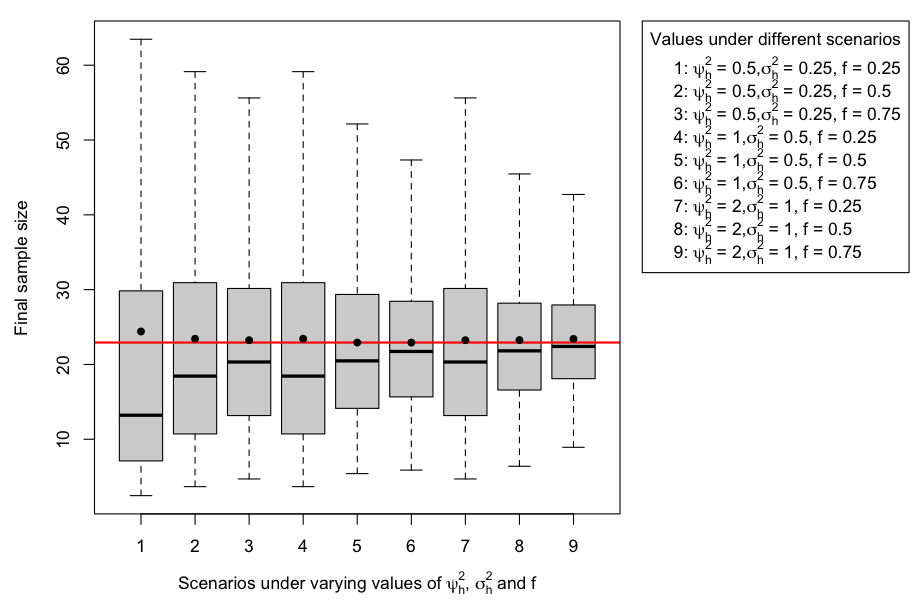
\includegraphics[scale=0.5]{Fig1}
    \caption{Mean reestimated sample sizes (mean indicated with black dot) and the variability under different $\psi_h^2$, $\sigma_h^2$ and \textit{f} compared to true model with $\psi_t^2 = 2$ and $\sigma_t^2 = 1$.}
    \label{fig:F1}
\end{figure}




%%%%%%%%%%%%%%% REFERENCES %%%%%%%%%%%%%%%
\newpage
\printbibliography

\newpage
\section*{Appendix}
\textbf{Future prospects} \\
\nodindent For the further course of the thesis the following steps will be taken: 
\begin{enumerate}
    \item Run more iterations (7500) for the different model scenarios proposed in this report to get more reliable results;
    \item Run entire trials under the scenarios proposed in the report and compare reestimated trials with N-of-1 trials with a fixed sample size in terms of power;
    \item Investigate the influence of sample size reestimation in N-of-1 trials on the type-I error rate;
    \item Look at the required number of patients \textit{and} cycles within patients to reliable reestimate the sample size. 
\end{enumerate}

\end{document}